\documentclass[table]{article}
\usepackage[utf8]{inputenc}
\usepackage{amsmath}
\usepackage{graphicx}
\graphicspath{ {images/} }
\usepackage{epstopdf}
\epstopdfDeclareGraphicsRule{.pdf}{png}{.png}{convert #1 \OutputFile}
\DeclareGraphicsExtensions{.png,.pdf}
\usepackage[final]{pdfpages}
\usepackage{tikz}
\usepackage{hyperref}
\usepackage{fancyhdr}
\setboolean{@twoside}{false}
\usepackage{tcolorbox}
\usepackage{tabularx}
\usepackage{array}
\usepackage{colortbl}
\tcbuselibrary{skins}

\tcbset{tab1/.style={fonttitle=\bfseries\large,fontupper=\normalsize\sffamily,
colback=yellow!10!white,colframe=red!75!black,colbacktitle=Salmon!40!white,
coltitle=black,center title,freelance,frame code={
\foreach \n in {north east,north west,south east,south west}
{\path [fill=red!75!black] (interior.\n) circle (3mm); };},}}


\usepackage{csvsimple,longtable,booktabs}
\usepackage{pdfpages}
\usepackage{multicol,caption}

\usepackage{lipsum}
\newenvironment{Figure}
  {\par\medskip\noindent\minipage{\linewidth}}
  {\endminipage\par\medskip}
\usepackage{float}
\newcommand{\code}[1]{\texttt{#1}}
\usepackage[a4paper, total={7in, 8in}]{geometry}
\title{Opportunistic Chunking in SeaFile Using the Duet framework}
\author{Ian Stewart-Binks, istewartbinks@gmail.com}
\date{December 2016}

\pagestyle{fancy}
\fancyhf{}
\rhead{Ian Stewart-Binks}
\lhead{CSC495 - Opportunistic Chunking}

\begin{document}
\maketitle

\newpage

\begin{multicols}{2}

\section{Abstract}

% Why did you do this study or project?
% What did you do, and how?
% What did you find?
% What do your findings mean?

Cloud-based file synchronization systems are becoming more ubiquitous in both personal and professional settings, and are used in both real-time collaboration environments and for backing up data. The performance of these systems is integral to their usability and correctness. In the following report, we identify that file synchronization systems that implement content defined chunking in the synchronization process and rely on inotify to detect file system changes as part of this process are performing redundant computations during chunking, which takes on average 67.08\% of the total synchronization time. In this report, we propose an opportunistic chunking algorithm that leverages the Duet framework to retrieve more granular file system event notifications. With these notifications, the algorithm reduces the amount of redundantly chunked data. We find that this algorithm performs up to 20 times faster than the conventional approach when used in select scenarios. This speed up can increase the usability of these applications and increase the likeliness of correctness.

\section{Acknowledgment}

I would like to thank a few people that have made this 3-month journey significantly more fruitful. I would like to thank two previous students that worked on setting the stage for the full implementation opportunistic chunking, Patrick Payne and William Kingsford: without inheriting their understanding of the colossus that is SeaFile, life would be much more tedious (and yet somehow still surprising - SeaFile always finds a way). I would like to thank Professor Angela Demke Brown and Professor Ashvin Goel for their immense guidance. I would like to thank George Amvrosiadis, who has made my inbox feel a little less lonely at 3 AM (but mostly I would like to thank him for the magnificent guidance he has provided me with over the past few months). Through the advice of these supervisors, I have found that I have been able to grow with regards to how I approach problems like the one we solve here: with clarity and curiosity. That result is perhaps more important than the ones we now present.

\section{Introduction}

Cloud-based file synchronization systems have recently seen a surge in usage and in popularity. As of March 2016, DropBox reports that a total of 500 million users \cite{dropbox-500} use their service, which is 100 million users more than their report from June 2015 \cite{dropbox-400}. As of February 2016, Apple reports that 782 million users use their iCloud product \cite{apple-782}. These systems synchronize files across different machines and often with a central server. They are used in both personal and professional environments for real-time collaboration and to backup data. For instance, these systems are frequently used for collaborative documentation writing at companies, interviewing candidates often across great distances, collaboration on assignments by students, among many other use cases. Moreover, a rising amount of the world's data is becoming digital, and this digital data is frequently backed up using these systems. Apple products have the ability to automatically sync data such as contacts or photos to the iCloud \cite{icloud-sync}. As the demand from users for cloud-based file synchronization systems erupts, the algorithms and frameworks that are used to implement these systems must keep up. Slow file synchronization services can impact usability and even correctness. Unfortunately, these algorithms are not always performant.\\

These services leverage the fact that they only need to synchronize files that have been modified, as it is redundant to synchronize an entire directory of files when only a subset of files has changed. To do this, these services rely on file notification frameworks. Moreover, we can extend this idea to a single file. If we know precisely what has been modified in a file, we need only update remote copies of that file with the data that have been modified, as it would be redundant to send over parts of the file that have not changed. Unfortunately, current file notification systems such as inotify \cite{inotify} in Linux, Kqueue \cite{kqueue} in Mac OSX, or the \code{FindFirstChangeNotification} API \cite{windows} in Windows only expose which files have been modified to the file synchronization system developer, and not where in the file these modifications have happened.\\

Substantial work has been done to create algorithms that reduce the amount of data that is sent across the network to synchronize a file. The low-bandwidth file system \cite{cdc} introduced a clever way to handle this problem of sending excess data: content defined chunking (CDC). CDC partitions the file into variable length chunks based on the file's data by using the Rabin rolling fingerprint \cite{rabin} to find such boundaries. The algorithm then produces a hash for each chunk and stores the chunk in a database using this hash as its key. Files are then represented as a series of hashes or keys. When a file is read, the database is queried for each of the file's hashes. When the file is synchronized, the file's hashes are sent over the network to the server. The server, which keeps a hash-to-chunk database itself, determines which chunks it doesn't have by comparing the client's hashes to its own. The server then requests only these chunks, which are the chunks that have changed.\\

\begin{Figure}
 \centering
 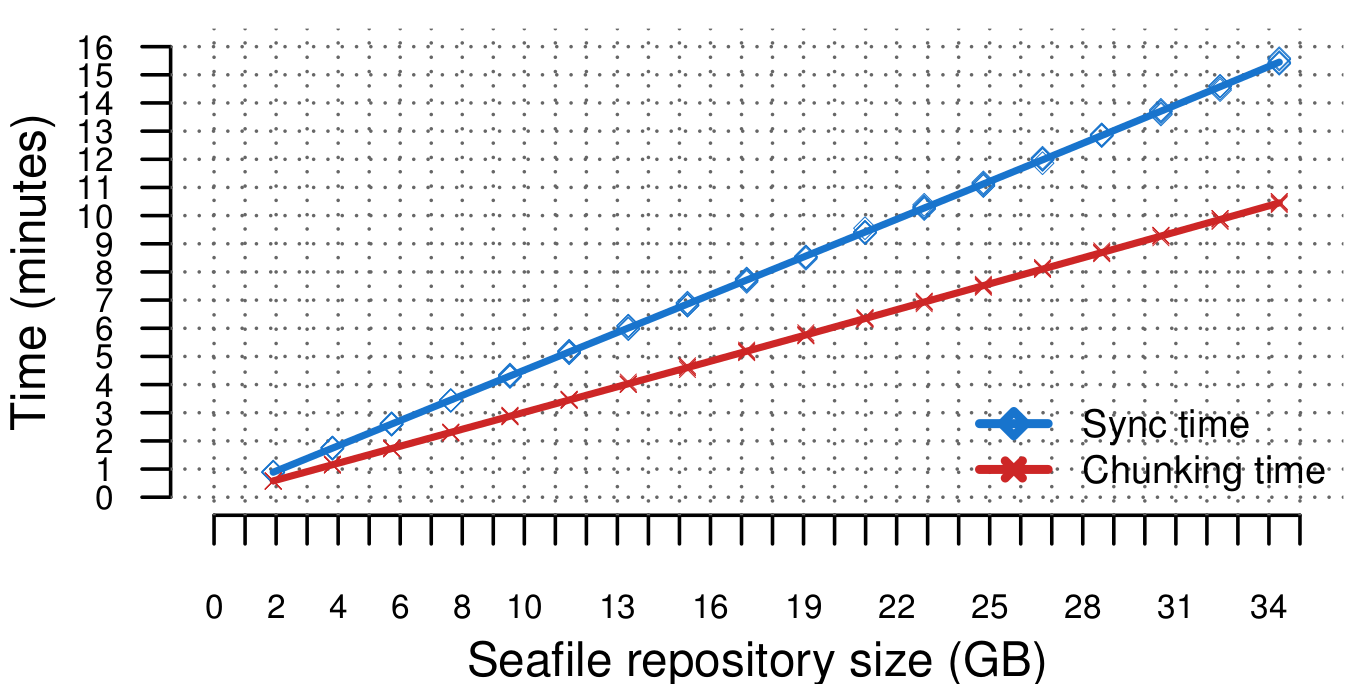
\includegraphics[width=\linewidth]{motivation_real.png}
 \captionof{figure}{SeaFile synchronization Time vs. Chunking Time (5 iterations)}
 \label{fig:SeaFileMotivation}
\end{Figure}

This alleviates the load on the network, and the time spent to synchronize redundant data but does not solve the whole problem. The CDC algorithm partitions the file based on file contents, which means that it must process the entire file, which incurs an unnecessary amount of I/O and computation. Even though it has alleviated pressure on the network, the algorithm currently relies on those file notification systems that only produce events at file-level granularity, and thus this algorithm can be improved. Moreover, we notice that the time that is spent on chunking dominates the synchronization time, taking on average 67.08\% of the entire synchronization time as shown in Figure \ref{fig:SeaFileMotivation}.\\

The Duet framework\cite{duet}, however, provides block granularity file event notifications. This framework allows the file synchronization software to register for notification events about activity in the Linux page cache. Thus, the file synchronization software can use the Duet framework to deduce which pages of a file have been modified, and thus which pages must be synchronized. We can leverage this information to only reprocess chunks that have been modified, thus reducing the total amount time spent on chunking and thus also reducing the total synchronization time.\\

In this report, we show how SeaFile \cite{SeaFile}, an open-source cloud-based file synchronization system that uses CDC for such purposes, can benefit from an opportunistic chunking algorithm that leverages the Duet framework to only reprocess chunks that must be reprocessed. In section 4, we describe the opportunistic chunking algorithm. In section 5, we evaluate the opportunistic chunking algorithm. In section 6, we outline future work that can be done to improve the significance of these results. In section 7, we conclude.\\

\section{Algorithm}

SeaFile's syncing algorithm mimics that of git. It uses the concept of local branches (on the client) and master branches (on the server), and uses git's notion of commits, repositories (which are synonymous with libraries), and merges \cite{SeaFile-sync-algo}. This part of the algorithm is less interesting for our purposes, though. Our primary target is SeaFile's use of content defined chunking (CDC).\\

SeaFile is implemented using CDC. When a file is 'chunked' \footnote{SeaFile uses the term 'block' instead of 'chunk' to refer to a chunk. We continue to call them 'chunks' in this report to distinguish them between 'blocks' that reside on disk, lest this report become very confusing at an unreasonable speed.}, its bytes are sequentially read in, and the Rabin fingerprinting scheme is applied to the most recently read 48 bytes. When the low 13 bytes of the fingerprint are 0, the chunking algorithm places a boundary after the final read byte. The bytes that we have read from the beginning of the file, or since the last time a boundary was placed, are called a chunk. Constraints are put on the size of a chunk: the size of a chunk must not be less than 2KB, or more than 4MB. These constraints are put in place for pathological cases, for instance when a file is entirely comprised of zeros. SeaFile claims that chunks are 1MB on average \cite{SeaFile-data-model}. SeaFile then writes these bytes to disk on the client. Although clients do store the hash representation of a file to communicate with a server, they only transiently store the chunked file data while they are transmitting it to the server: it is not stored permanently. If it was, then SeaFile would force the user to only be able to fully utilize half of their file system, the other half would be used for the chunk database. Once chunk data is transmitted to the server, it is erased from the client. The original files are all the client needs.\\

These chunks are then stored in a chunk database on the server: a key value store with the SHA1 hash of the chunk as the key, and the data of the chunk as the value. Files are then represented as a sequence of these hashes. When a file needs to be reconstructed, say if a new client is downloading the file from the server, the file will be reconstructed by mapping hash id to its data from the chunk database.\\

Content defined chunking has three primary purposes. First, it is used to limit the amount of data that is sent between the client and the server when a file is synchronized. Consider a 40MB file on the client that is synchronized with the server, and let's imagine we're using a file synchronization system that doesn't use CDC. Suppose a user modifies a single byte of a file. We would likely need to transfer the newly modified file to the server such that the client and the server are synchronized. That is quite a bit of redundant data that is being sent across the network. A clever solution to this problem would be to just send the block that the user modified. However, if a user inserts data into the file, all data in subsequent blocks are shifted along in the file, and each subsequent block is technically modified. In this second example, we would still be sending redundant data. With content defined chunking, the client can send just the chunk that has been modified to the server. Should a user insert into the file, subsequent chunks won't be modified because the chunks are partitioned on content, not on size like normal file system blocks are\footnote{However, there is a rare case in which the modification of one chunk forces all subsequent chunks to change. In the pathological case when a chunk is 4MB large, and we can't grow the chunk any further, if we insert data into this chunk, we move the data that are at the end of the chunk to the next chunk. Thus, the next chunk must be rechunked. Should that chunk also be at the 4MB size limit, its subsequent chunk will need to be rechunked, and so forth.}. Second, CDC benefits from deduplication. Consider the case when the server is storing two copies of a file. The chunking algorithm will partition both files in the exact same way since they have the same content. However, the chunk database will only contain one entry per chunk, thus storing the duplicated content only once. Third, since the data are now separated, they can be transferred in parallel. SeaFile implements this if the client is synchronized with several servers, but does not use parallelism when syncing with a single server\cite{SeaFile-data-model}.\\

When a file is modified, an inotify event is generated. SeaFile performs different actions based on what type of event is generated. If both events \code{IN\_MODIFY} and \code{IN\_CLOSE\_WRITE} are detected, SeaFile infers that a file has been changed on the client and must be synchronized with the server. SeaFile then inserts an event into the event queue to synchronize the file. Once this event is processed, SeaFile performs the aforementioned chunking algorithm on it, and sends new chunks to the server. Note that each file is chunked and sent separately.

\subsection{Opportunistic Chunking Overview}

When a file is rechunked (that is, the file is chunked but this is not the first time we've chunked it), the entire file is read into memory and each byte is reprocessed. If only one chunk of a file has changed and needs to be updated with the server, SeaFile still reprocesses the entire file and reproduces chunks that we have already produced. Thus, SeaFile processes a lot of data redundantly.\\

We have built an opportunistic chunking algorithm on top of a modified Linux kernel that includes the Duet module. The Duet module hooks into the page cache and provides events about what blocks of a file have been added to the cache, modified, flushed from the cache, etc. For our algorithm, we care about events that let us know which pages are dirty. With these events, we can infer where in a file modifications have occurred.\\

The general idea of the algorithm is simple. When a file is modified on disk, we look at which chunks have been changed, and only rechunk those chunks to send to the server. We leave the other chunks of the file alone: they have not been modified, and do not need to be reprocessed. There are corner cases, which we will explore in the implementation details.

\subsection{Implementation}

The implementation of opportunistic chunking can be broken down into three phases: the recording phase, the reading phase, and the opportunistic chunking phase.

\subsubsection{Preamble}

We register for Duet events at the same time that inotify watches are added. We deregister for Duet events when inotify watches are removed. So far, this has worked well, as SeaFile adds and removes inotify events to enable/disable the syncing feature.

\subsubsection{The Recording Phase}

The recording phase is only executed once for a file: when the file is first synced by SeaFile. This phase has no prior information about the file, and is meant to produce the starting offsets at which each chunk resides in the file. These offsets are necessary for opportunistic chunking, as we will soon see. SeaFile uses files to persist file metadata, such as repository, repository version, and hash representation of the file, and uses \code{JSON} to represent this information. Naturally, we store the offset information for each chunk in the file in its corresponding metadata file. This way, since the file metadata is easily accessible during chunking, so is the offset information. Moreover, the data persists even when SeaFile is restarted, so the recording phase only need be invoked once per file. We chunk the entire file when it is first created since the server has no chunk data corresponding to the given file. The offset metadata is updated when a chunk is written to disk. As such, when we read Duet events in the future, we can tell which chunks have been changed by seeing which modified blocks belong to which chunks.

\subsubsection{The Reading Phase}

SeaFile uses a separate thread to \code{select} on inotify and Duet events. For our purposes, this thread needs to read in events, and needs to provide information about what blocks of a file have changed. In our implementation, we consider such blocks as 'live'.\\

When the thread receives Duet events, it reads in each event and appends it to a file specific array. This array keeps the offsets of each block that has been modified in the file. These arrays are stored in a hash table whose keys are file paths and values are the corresponding live block offset arrays. We use the \code{GArray} and \code{GHashTable} data structures for the implementation (the \code{GArray} is not the best data structure for the implementation, we discuss this in future work). These arrays are then made available to the chunking thread through a shared hash table containing data structures identical to the aforementioned hash table. The event processing code operates on thread local hash tables when processing Duet events and then copies the final result to the shared hash table to alleviate contention for the shared hash table locks\footnote{The majority of the code for this phase resides in the file \code{daemon/wt-monitor-linux.c}.}.\\

\subsubsection{The Opportunistic Chunking Phase}

During the chunking phase, we collect the data that are made available to use from previously executed: the chunk offsets from the recording phase and the live block offsets from the reading phase/a previous opportunistic chunking phase. We then construct a bitmap, the live chunk list, by mapping the live block offsets onto the chunk offsets. Since we need to find the first chunk offset that is less than or equal to the block offset, we iterate from the final chunk offset to the first chunk offset. In this bitmap, a 1 means that data in that chunk were intentionally modified \footnote{The implementation actually always considers the final chunk live in the case that data are appended. This can be improved on significantly, which we touch on in the "Evaluation" and "Future Work" sections}.\\

We begin chunking by iteratively inspecting the live chunk bitmap. If we find a zero, we write out the corresponding chunk metadata (the offset and its hash). The data for this chunk has not changed, so we do not need to reprocess it. We then move onto the next element of our live chunk bitmap. If we find a 1, we chunk the chunk that the index corresponds to. When we process this chunk, it will produce a chunk boundary using the Rabin Fingerprinting scheme. If this chunk boundary lies in the exact location of an existing chunk boundary (one that we retrieved from the offsets of the file), then we stop chunking and return to inspecting the live chunk bitmap for the next live chunk. If the chunk boundary is a new boundary, we write this boundary to the metadata. We then chunk until we lay an existing chunk boundary before returning to our inspection of the live chunk bitmap\footnote{The majority of the code for this phase resides in the files \code{common/cdc/cdc.c}, \code{daemon/repo-mgr.c}, and \code{daemon/fs-mgr.c}.}.

\subsection{Edge Cases}

There are several edge cases that we need to account for. We go through the cases when data are appended to a file, chunk size limitations in pathological scenarios, blocks that create or erase boundaries, and blocks that belong to two chunks. However, there is a limitation in the algorithm regarding blocks that belong to two chunks.

\begin{itemize}
    \item \textbf{Appended Data}
    
        The implementation accounts for the case when data are only appended to the file. Should data be appended to a file, the final chunk must be rechunked, as it has changed. Since we find the first chunk that has an offset that is less than the block offset, and we check chunk offsets from largest to smallest, any live blocks that represent appended data will map to the final chunk in the live chunk list \footnote{This is handled different in the implementation. See 'Future Work' for more details, specifically \textit{Fix Opportunistic Chunking Algorithm}}.

    \item \textbf{Chunk Boundary Size Cases}
    
        SeaFile enforces that chunk boundaries not exceed 4MB or be smaller than 2KB. That means that if the Rabin Fingerprinting scheme tells SeaFile to place a boundary within 2KB of a previous boundary, the new boundary will be discarded and that if a boundary is not found before 4MB have been read in for chunking, a boundary will be placed after 4MB. This case necessitates careful inspection.\\

        If we start chunking at a given offset, and a new boundary is found within 2KB of that offset, our algorithm will discard that offset. If a new boundary is placed within 2KB of a future existing boundary, thus forcing the old boundary to cease to exist, our algorithm will not stop chunking because we have not yet laid down a chunk boundary at the same location of an old chunk boundary. If data are inserted into a chunk that is of maximum size, we handle this case similarly by chunking until we reach a familiar chunk boundary.

    \item \textbf{Nested erased/created chunk boundaries}
    
        Should a block create or erase a chunk boundary, we chunk until we find a familiar block offset. During chunking, we are required to manage some indices. These counters require careful thought in the implementation to avoid bugs when dealing with edge cases. In order to lay the file out sequentially, when we chunk a file we need to know what index the chunk is in the file. For instance, if we process chunk 4, its index in the sequence of hashes that represent the file will be 3. Similarly, we need to use a counter to keep track of which chunk we're inspecting in the live chunk bitmap. Ideally, these two counters would be identical, however, we cannot assume that this is the case. Consider the following case: we have a bitmap of 0100, indicating to us that the 2nd chunk has changed. Our index into the bitmap is 1, and the next chunk that will be written will have index 1. When chunking the second chunk, the new modifications actually place a boundary in the middle of the chunk. When this happens, we write out two chunks and increment the file's index by 2. So, the index into our bitmap will be 2 on the next iteration, and the block number of the chunk we will be 3. Note that we can also eliminate a boundary with a modification, in which case the live chunk index will increment by 2, while the file index increments only by 1.

    \item \textbf{Blocks belonging to two chunks}
    
        Should an entire block of a file be modified, and should that block start on one chunk, and ends on another, both chunks will need to be rechunked. It is likely the case that the chunk boundary will be erased, as the 48 bytes preceding the chunk boundary will likely no longer trigger a boundary. However, if they do still trigger a boundary, we will place a boundary at the same location as a previous chunk boundary, and we will not chunk the subsequent chunk, leading to incorrect behaviour. This is a limitation of the algorithm that must be updated.

\end{itemize}

\section{Evaluation}

\subsection{Methodology}

To evaluate SeaFile, we first implemented a timing system within the original code. This timing system evaluates the following metrics:

\begin{itemize}
    \item Setup Time: The time SeaFile spends initializing.
    \item Total Bytes Read: The total number of bytes read during the synchronization process (both for chunking and other purposes).
    \item Total Bytes Written: The total number of bytes written during the synchronization process (both for chunking and other purposes).
    \item Total Bytes Chunked: The total number of bytes chunked, i.e. the total number of bytes read in for chunking.
    \item Total Time Spent Chunking: The total time spent chunking.
    \item Total Time Spent Synchronizing: The total time spent from when the setup completes to when the repository transitions to a 'synchronized' state and all files are chunked.
    \item CPU Time User: The total amount of CPU cycles spent in user space during the chunking process.
    \item CPU Time System: The total amount of CPU cycles spent in system space during the chunking process.
    \item Metadata Time: The total time spent loading metadata that is used in the chunking algorithm.
\end{itemize}

These metrics are included in all of our tests, even if the numbers are not represented in the graphs in the evaluation section.\\

The setup timer is started at the beginning of the daemon's \code{main} function, and is stopped once SeaFile's internal 'started' state is set to \code{TRUE}, which happens to be directly after all watches on each repository's directories has been registered. Once SeaFile's internal 'started' state is set to \code{TRUE}, we then also begin the global timer that is used to measure the time it takes SeaFile to synchronize a set of files. We also initialize all other fields to 0 at this point.\\

The CDC code is placed within a single function. The chunking timers are started once the function is entered, and are stopped once the function has finished. The CPU Time User and CPU Time System are started are also managed in this way. When bytes of a file have been read within this function for the purpose of chunking, the total number of read bytes is added to the \textit{Total Bytes Chunked} counter.\\

The opportunistic algorithm performs metadata loading that the original chunking algorithm does not. We measure the time it takes to load the metadata using the \textit{Metadata Time} timer.\\

We implemented a microbenchmark to evaluate SeaFile. The microbenchmark operates by first generating a set of files. These files generate random content using \code{urandom}, a Linux kernel random number generator. These files are synced to the central repository by SeaFile. The timers are not collected during this initial syncing period. SeaFile is then killed and we subsequently modify a given location in each of the files. The location we choose to modify, along with the justification for the choice, will be discussed in the Evaluation section. SeaFile is then started. In both Vanilla SeaFile and SeaFile with Duet, inotify watches are placed on each file in the repository. After the watches have been added, SeaFile adds a \code{WT\_EVENT\_SCAN\_DIR} event to its event queue. This event causes SeaFile to scan each file in the repository and to add it to the index. This forces SeaFile to chunk files that have been modified such that it can synchronize with the server. This presents a good opportunity to then compare our opportunistic chunking algorithm with the vanilla chunking algorithm.\\

When the microbenchmark has generated all of the files and then stopped SeaFile, it keeps Duet alive to listen for modification events on these files. SeaFile is then started again, which registers a task with Duet to watch the repository. We then disable SeaFile's auto-syncing mechanism, which deregisters Duet. We now drop the caches such that SeaFile must bring the files in from disk to chunk them: this better exhibits the problem of doing so much I/O \footnote{There is a problem with the way we drop caches here. We don't drop them after the modifications have been made, which would be ideal. We describe the problem in the 'Evaluation' section, \textit{The Cache Dropping Anomaly}}. The files are each then individually modified in a location and fashion specified by the given experiment. Auto-syncing is re-enabled, which registers Duet again, and spawns another \code{WT\_EVENT\_SCAN\_DIR} which causes all files to be chunked. When the directory scanning event decides to chunk files, it uses our opportunistic chunking algorithm along with the events that have been collected from Duet. We disable auto-syncing while we modify the files because we don't want the SeaFile chunking process to have to compete for resources with the microbenchmark as this has shown to heavily influence our results in preliminary tests.\\

In order for us to accurately time the end of the synchronization process, we need to know when SeaFile has finished chunking all files and those chunks have been uploaded to the server. In order to do this, we keep track of how many files have been chunked. Once the number of chunked files reaches the number of files in our repository, and SeaFile's state has transitioned back to 'synchronized', we stop our global timer.\\

The microbenchmark also provides correctness functionality. The correctness functionality first synchronizes a given directory as per the specification above, and then checks it out from the server in a separate directory. It asserts that both repositories are identical.\\

In our experiments, we have used two machines from the Sysnet cluster. Their specifications are as follows:


    %\begin{tabular}{|l|l|}
    \rowcolors{1}{blue!30}{white}
    \begin{tcolorbox}[enhanced, width=1\linewidth, tabularx={>{\centering\arraybackslash}l|>{\centering\arraybackslash}X}, title={Server Specifications}]

      CPU & Intel(R) Xeon(R) CPU E5-2650 \\
      \hline
      CPU Speed & 2.00GHz \\
      \hline
      \# CPUs & 32 \\
      \hline
      Cores/CPU & 16 \\
      \hline
      Memory (RAM) Size & 32 GB \\
      \hline
      Memory (disk) Size & 140 GB \\
      \hline
      Distribution & Ubuntu 16.04 LTS \\
      \hline
      Kernel Version & Linux 4.4.0-36-generic \\
      \hline
      SeaFile Version & 6.0.5 (server, Linux) \\
      \hline
    \end{tcolorbox}
    \captionof{table}{Server Specifications}
    
    \rowcolors{1}{blue!30}{white}
    \begin{tcolorbox}[enhanced, width=1\linewidth, tabularx={>{\centering\arraybackslash}l|>{\centering\arraybackslash}X}, title={Client Specifications}]
      CPU & Intel(R) Xeon(R) CPU E5-2650 \\
      \hline
      CPU Speed & 2.00GHz \\
      \hline
      \# CPUs & 32 \\
      \hline
      Cores/CPU & 16 \\
      \hline
      Memory (RAM) Size & 32 GB \\
      \hline
      Memory (disk) Size & 140 GB \\
      \hline
      Distribution & Ubuntu 16.04 LTS \\
      \hline
      Kernel Version & Linux 4.7.0+duet-e0e18d6 \\
      \hline
      SeaFile Version & 6.0.5 (client, Linux) \\
      \hline
    \end{tcolorbox}
    \captionof{table}{Client Specifications}


The server is using Maria DB version 2.3.1 for the chunk database. This is the recommended database on the SeaFile setup guide.

\subsection{Overview of Evaluation}

We perform the tests on a single repository. Upon each iteration of the test, we generate 50 more files than the previous iteration, up to a maximum of 900 files. Each file is comprised of 10,000 data blocks of 4096 bytes, or 40,960,000 bytes (approximately 40MB). Each file is modified and synchronized with the central server on each iteration of the test.

\subsubsection{In-place vs. Insertion Scenarios}
The opportunistic chunking algorithm works well. When a block is modified in the middle of a file, we are guaranteed to only start chunking from the beginning of the chunk in which that block lies. When the modification happens at the beginning of the file, it is likely that we'll only chunk the first chunk, barring pathological cases. However, this is not always true. If we modify the beginning of the file in place such that data are changed and not inserted, we will likely only chunk the first chunk, but if we insert into the file, we chunk the chunk on which that block lies as well as every subsequent chunk. This is because when data are inserted into a file, all subsequent data are shifted across the file's blocks in the file system. As such, all subsequent blocks are considered modified. Duet reports these blocks as being modified, as it should. We thus evaluate Opportunistic Chunking against SeaFile in these two scenarios: the in-place scenario and the insertion scenario. This limitation is significant, as we can imagine that user modifications are likely going to insert data into the file. However, there are cases in which this is not the case, such as virtual disk images. %To emulate virtual disk images, we run the tests on a single large file (25GB). The other tests are each run on a set of files ranging from 50 to 900 files in increments of 50 files. We choose a large number of files to exhibit the scalability of chunking with and without opportunistic chunking. Finally, we also measure the time it takes to load the data necessary for opportunistic chunking.

\subsubsection{Incomplete Results}

        The evaluation attempts to discuss all elements of the experimental setup and experiment decisions. However, due to anomalous behaviour and time constraints, the evaluation suffers.

\begin{itemize}
\item \textbf{The Cache Dropping Anomaly}

        We tried very hard to build a very strong experimental setup. One element of this setup was that we wanted to have no data in the cache when we measure how long it takes to chunk. We weren't able to do this.
        
        The steps in our experimental setup are to:
        \begin{enumerate}
            \item Start SeaFile
            \item Generate files on client
            \item Sync All files with server
            \item Stop SeaFile
            \item Start SeaFile
            \item Disable auto-sync
            \item Make modifications to files
            \item Drop caches (\code{sync} + \code{echo 3 >> /proc/sys/vm/drop\_caches}) \footnote{We have tried all levels of cache dropping and were not successful}
            \item Enable Auto-sync
            \item Sync (measure chunking time)
        \end{enumerate}
        
        We weren't able to successfully drop the caches in the setup with Duet. The events are mysteriously lost. We get similar results when we \code{fsync} the files after modification. We have written scripts to emulate this behaviour outside of SeaFile, and the events aren't lost. We have looked into this extensively, but have not found anything yet. We suspect that SeaFile is doing something in the background that doesn't play nicely with Duet.
        
        To combat this, we drop the caches after we've generated the files, but before we've modified them. This way, we assume that there only exists one page in the cache at chunking time, which should be negligible given that the files are comprised of exactly 10,000 blocks in our experiment.
        \item \textbf{Implementation Limitation}
        
            The implementation of the algorithm always considers the final chunk as live to account for the case when data are appended to the file. This is not the best way to do this, and our results for the in-place beginning experiment suffer - Duet performs twice as badly than in the in-place end scenario because we are chunking twice the amount of chunks (one of which does not need to be chunked).
        \item \textbf{More Results}
        
            We have spent a lot of time analyzing the anomalous behaviour, and postponed running the experiments until we had the experimental setup to our liking. We were not able to uncover the mystery behind The Cache Dropping Anomaly, and as such spent too much time on it before deciding to go ahead with a less than ideal setup.
\end{itemize}
\subsection{In-place Scenario}

We split up the evaluation of the in-place scenario into beginning and end to show that SeaFile does perform well if data are modified anywhere in the file. This is in contrast to an earlier implementation of opportunistic chunking that does not support modifications at the beginning of the files well.

\subsubsection{End}

In the first in-place scenario, we modify a single byte of the final block of each file in the directory. On average, Duet spends 67.20\% of the total synchronization time chunking. On average, opportunistic chunking completes chunking in 4.45\% of the time it takes vanilla SeaFile to chunk the same amount of data, and completes the total synchronization in 6.98\% of the time that it takes SeaFile. These results indicate that opportunistic chunking performs almost 20 times better than vanilla chunking.\\
%Average fraction of chunking time compared to sync time 67.20%
%Average fraction of chunking improvement with Duet 4.45%
%Average fraction of global improvement with Duet 6.98%

\begin{Figure}
 \centering
 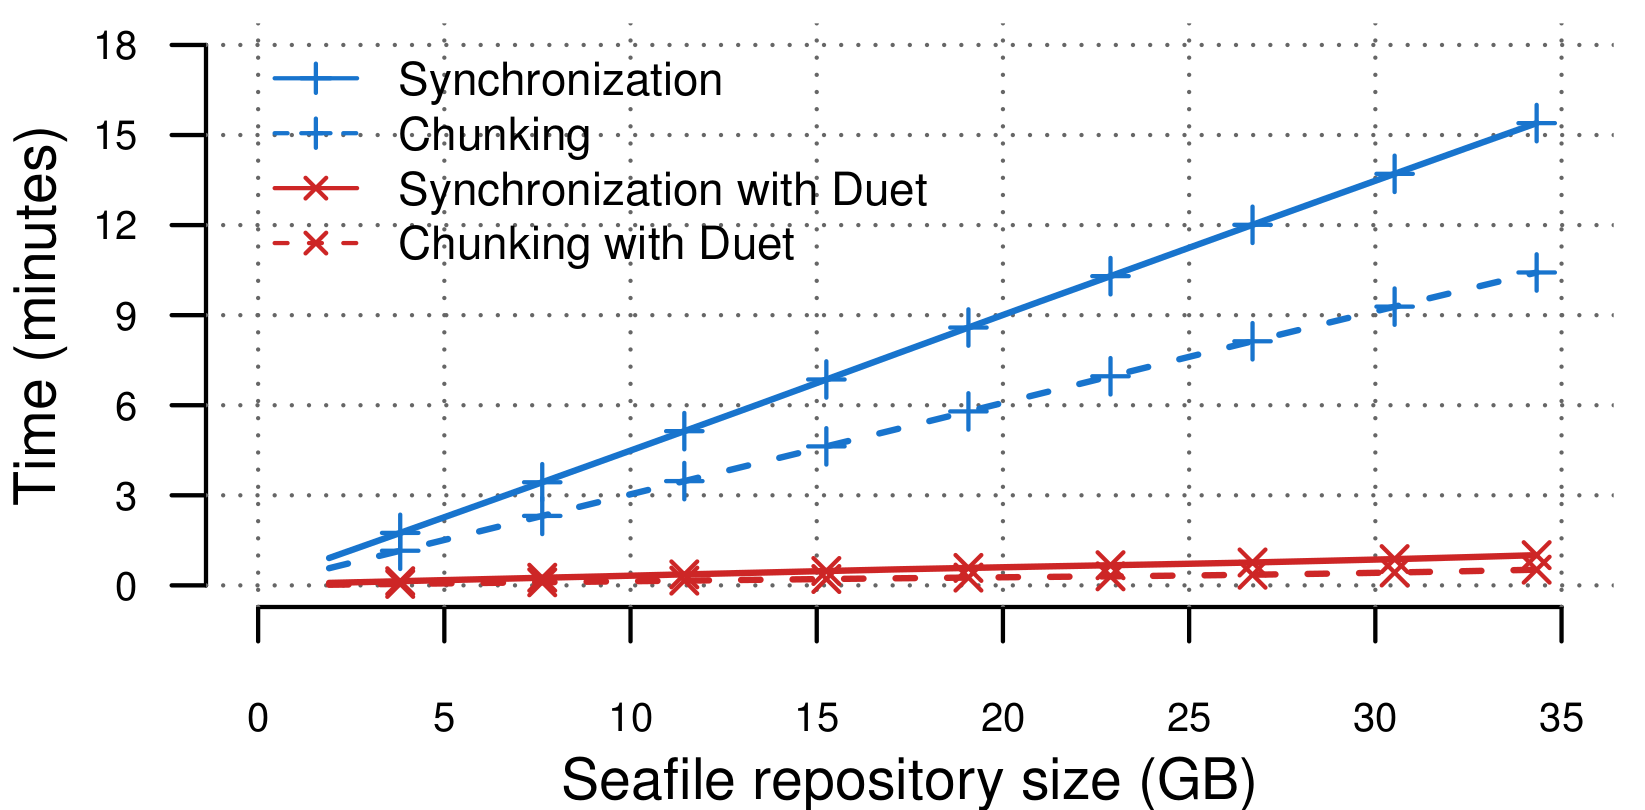
\includegraphics[width=\linewidth]{duet_in_place_end.png}
 \captionof{figure}{SeaFile Sync/Chunking Time with and without Duet (in-place, end) (1 iteration)}
 \label{fig:SeaFileInPlaceEnd}
\end{Figure}

As we can see in Figure \ref{fig:SeaFileInPlaceEnd}, SeaFile performs significantly better with opportunistic chunking. The results scale linearly, and chunking takes approximately the same fraction of the total synchronization time regardless of the size of the repository.\\

Since SeaFile limits chunks to be 4MB large, our files are guaranteed to be partitioned into more than 10 chunks. On average, SeaFile states that chunks should be around 1MB in size\cite{SeaFile-data-model}, meaning our files on average should have 40 chunks. Opportunistic chunking chunks only 1 chunk in this case, so we could expect that the total speedup we measure to be much greater than 20 times that of vanilla chunking. Opportunistic chunking does spend a fair amount of time preparing and calculating metadata, which likely takes a non-negligible amount of time, but perhaps not as much time as we see being spent here. To better understand these numbers, it would be beneficial to calculate how many chunks files have on average. While debugging the microbenchmark, I did notice that files had around 30 chunks in total. This number is not reliable because it only represents a few files, however it provides a hint that we don't fully understand how much of a speedup we can expect.\\

We have run profiling tools on SeaFile with opportunistic chunking to understand where time is lost in the program. Unfortunately, given the distributed and multiprocess nature of SeaFile, \code{callgrind} reports are unreliable with the parameters it's been run with, and \code{perf} may take a little more time to set up with the modified kernel. SeaFile has been run with \code{gprof}, which tells us how many times a function has been called. Unfortunately, it neglects to give us any other information, which, to the best of my knowledge, indicates that the executable being profiled, \code{seaf-daemon}, isn't shut down correctly by the \code{seaf-cli} client Python script. Note, however, that the SeaFile developers use \code{gprof} to profile their code, and as such support for \code{gprof} is already built into the program. The numbers we get from SeaFile are shown in figure \ref{fig:GprofResults}.

\begin{Figure}
 \centering
 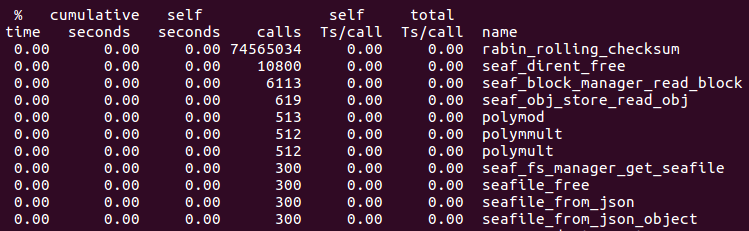
\includegraphics[width=\linewidth]{results_gprof.png}
 \captionof{figure}{Top gprof results of SeaFile with opportunistic chunking, run with 100 files each with 10000 blocks (in-place end scenario)}
 \label{fig:GprofResults}
\end{Figure}

A 20x speedup is a favourable result: it takes vanilla SeaFile ~15 minutes to synchronize small modifications on almost 35GB of data, whereas it takes SeaFile with opportunistic chunking less than a minute.

\subsubsection{Beginning}

In the second in-place scenario, we modify a single byte of the first block of each file in the directory. On average, opportunistic chunking spends 67.09\% of the total synchronization time chunking. Duet completes chunking in 10.46\% of the time it takes vanilla SeaFile to chunk the same amount of data, and completes the total synchronization in 11.57\% of the time that it takes SeaFile.\\

%Average fraction of chunking time compared to sync time 67.09%
%Average fraction of chunking improvement with Duet 10.46%
%Average fraction of global improvement with Duet 11.57%

\begin{Figure}
 \centering
 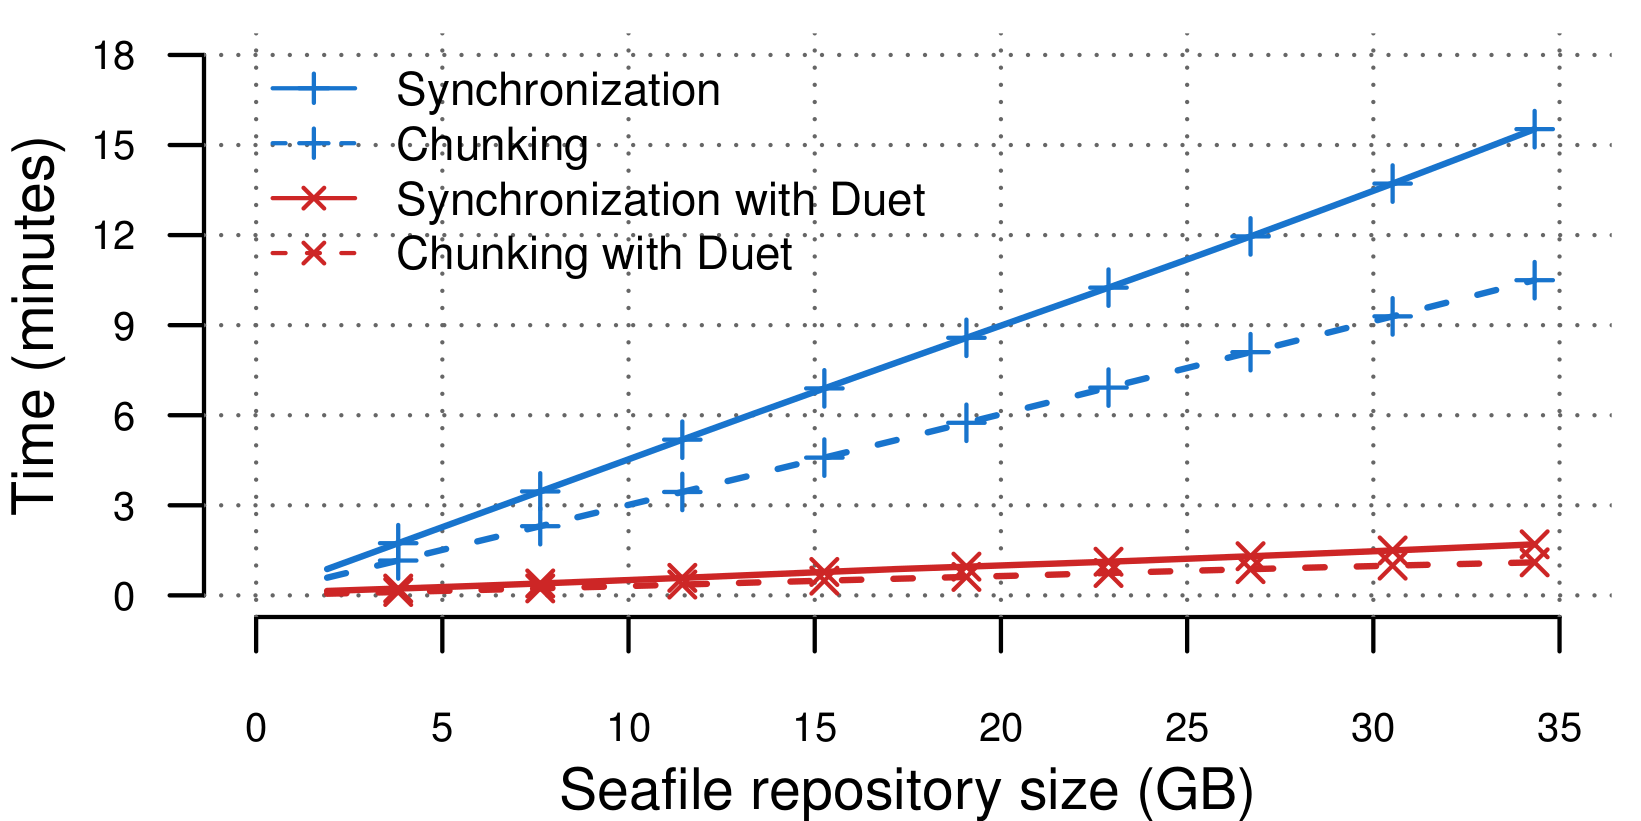
\includegraphics[width=\linewidth]{duet_in_place_beg.png}
 \captionof{figure}{SeaFile Sync/Chunking Time with and without Duet (in-place, beginning) (1 iteration)}
 \label{fig:SeaFileInPlaceBeginning}
\end{Figure}

As we can see in Figure \ref{fig:SeaFileInPlaceBeginning}, SeaFile performs significantly better with opportunistic chunking again. The results scale linearly, and chunking takes approximately the same fraction of the total synchronization time regardless of the size of the repository. The results appear to be twice as slow as the in-place end scenario, and for good reason. The opportunistic algorithm considers the final chunk to be 'live' to account for appended data (which, as has been expressed several times, is not the best way to account for this case). Thus, we chunk twice the amount of data in this scenario compared to the in-place end scenario. These results match the expectation.

\subsection{Insert Scenario}

%Average fraction of chunking time compared to sync time 67.20%
%Average fraction of chunking improvement with Duet 148.15%
%Average fraction of global improvement with Duet 118.28%

The following scenario exhibits the worst-case scenario for opportunistic chunking: when data are prepended to the file, thus generating events for every single block of the file.

\begin{Figure}
 \centering
 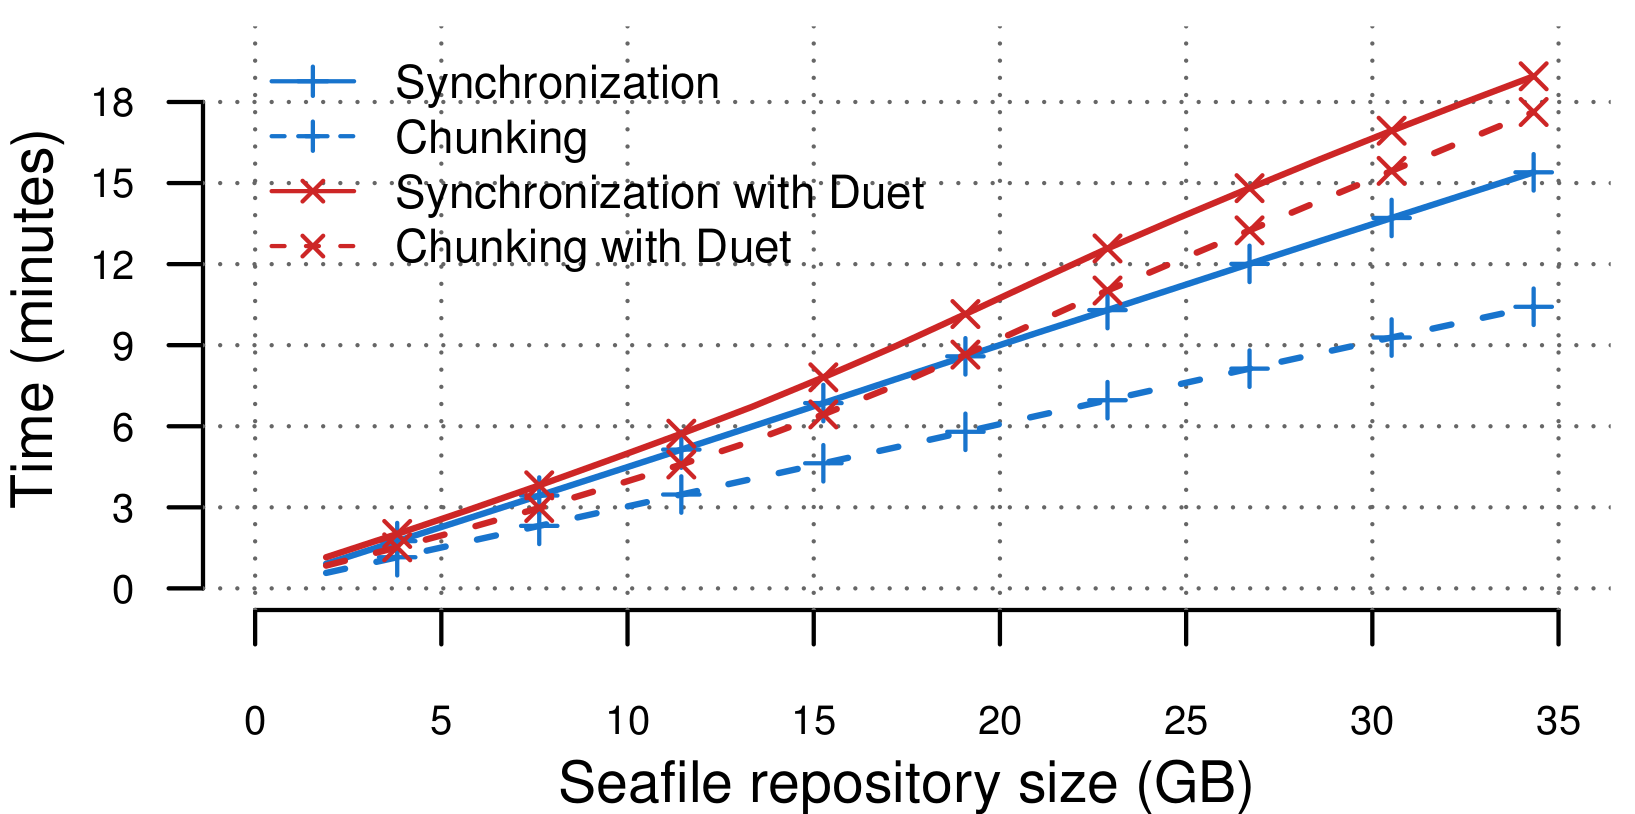
\includegraphics[width=\linewidth]{insert.png}
 \captionof{figure}{SeaFile Sync/Chunking Time with and without Duet (insert) (1 iteration)}
 \label{fig:SeaFileInsert}
\end{Figure}

The results in Figure \ref{fig:SeaFileInsert} show that opportunistic chunking performs much worse in the insertion scenario than it does in the in-place scenario. Moreover, given the amount of overhead that opportunistic chunking requires in order to work, it performs worse than vanilla SeaFile when both chunk the same amount of data. The total time to chunk the files is 148.15\% more than that of vanilla SeaFile on average. The total synchronization time of opportunistic chunking is 118.28\% of the total time of vanilla SeaFile.

The above results are unexpected. Opportunistic chunking takes up 87.52\% of the total synchronization time, which is significantly different than the 67\% result yielded from vanilla SeaFile, and opportunistic chunking in early test cases. However, it may be the case that there is parallelism going on behind the scenes that cause the increased chunking time to overlap with synchronization operations. This evaluation will need to be continued and heavily scrutinized.

\subsection{Metadata Overhead}

SeaFile with opportunistic chunking spends a fair amount of time loading metadata. We calculate the metadata load time as being the time it takes to locate the metadata file on disk and read the chunk offsets into memory. For the in-place end experiment, opportunistic chunking spends 9.2\% of the total synchronization time loading metadata for chunking on average. In the insert scenario case, opportunistic chunking spends 0.25\% of the total synchronization time loading metadata. This result is expected to grow with the number of files in the repository as well as the size of the files.

\section{Future Work}

The goal of this work is to prove that Duet can be used to improve the performance of widely used applications in significant and meaningful ways. This report moves us forward, but there are several things we need to do to make these results more meaningful. We list these here:

\begin{itemize}
    \item \textbf{The Cache Dropping Anomaly}
    
        We need to fix the experimental setup and rerun the results with the caches dropped. The Cache Dropping Anomaly is discussed in the Evaluation section.
        
    \item \textbf{File Access Patterns}
    
        Our experimental setup modifies files at the beginning and end of a file with randomly generated data to show the power of opportunistic chunking, but it's unclear what that means for normal users. As far as I understand, work has been done with duet-telemetry on trying to figure out how users access files with cloud-based file synchronization systems, but we need more. It might also be helpful to add more experiments that show how much speedup users can typically expect.
        
    \item \textbf{Improve Metadata Overhead Performance}
        
        When collecting events from Duet, we store them in a \code{GArray}. The \code{GArray} has negligible performance impact on the tests - we only ever receive two events per block for the test (\code{DUET\_PAGE\_DIRTY} and \code{DUET\_PAGE\_FLUSHED}, we would only receive one event when registered for level-triggered events), and as such never have unbounded duplicate blocks. The initial implementation used the \code{GArray} because it was thought that we would only be processing one event, in which case the tests would not suffer the performance hit because we would perform the same, or better, than an implementation using a balanced BST. Since we do see duplicate events, we likely incur a performance hit in the tests. In practice this will hurt our performance a lot. We should use a \code{GTree} to improve the performance of event collection. An implementation is currently underway, and is not yet complete due to the amount of code that the \code{GTree} API forces us to modify in SeaFile.
        
    \item \textbf{Fix Opportunistic Chunking Algorithm}
    
        One problem with the opportunistic chunking algorithm is that it always considers the final chunk live in order to deal with appended data. The algorithm section provides an implementation that works much better. Another problem resides in the 'Blocks belonging to two chunks' edge case mentioned in the Algorithm implementation. This is an improbable case, but must be fixed regardless.
        
    \item \textbf{Level Triggered Duet}
    
        Level-triggered event support has recently been added into Duet. The current opportunistic implementation uses edge-triggered Duet because it only ever reads events once for the tests. This is simple to implement: we need to recompile the kernel with level-triggered Duet, and change our Duet register flags from \code{DUET\_PAGE\_DIRTY}/\code{DUET\_PAGE\_FLUSHED} to \code{DUET\_LEVEL\_DIRTY}.
        
    \item \textbf{Using Select}
    
        Duet should be the sole file system event notifier in SeaFile. This is a very simple change: Duet is already FD based, so all we likely need to do is remove the inotify fds from the select fd set and add the Duet fd.
        
        One question still remains. SeaFile syncs a file once it has been written to \textbf{and} closed. Duet does not provide this functionality.
        
    \item \textbf{Getting Inotify Metrics}
    
        One of the powerful characteristics about Duet is that it watches recursively. Inotify does not, which means that SeaFile implements a lot of complex code to recursively add watches. Moreover, inotify can only handle so many events, so it then needs to keep an internal notification queue in the event of overflow. This is bad, and SeaFile's performance likely suffers.\\
        
        We need to remove inotify from SeaFile (although, see comment in 'Using Select'), and we need to measure how much of a speedup using Duet provides.
        
    \item \textbf{Better Profiling}
    
        We should better understand where time is spent in SeaFile and should use performance testing tools to do so. This report attempts to use \code{perf}, \code{callgrind}, and \code{gprof} to understand which functions may be the bottlenecks, but does not yield useful results.
        
    \item \textbf{Parallelism}

        It is possible to infer exactly which chunks will or may be changed based on the offsets of both the existing chunks and the modified blocks of the file. This means that chunks can be processed in parallel. It may be worthwhile, and would certainly be fun, to explore this. Note, however, that there may be challenges in writing chunks in parallel.

\end{itemize}

\section{Conclusion}

The above report exhibits the power that Duet can bring to applications like SeaFile, which could ultimately affect hundreds of millions of cloud-based synchronization system users. We see that using Duet over inotify can speed up the total synchronization time of SeaFile by 20x. However, there is still work that needs to be done to evaluate the insert scenario and to reduce the amount of overhead that opportunistic chunking warrants in its current implementation.


\end{multicols}
\begin{thebibliography}{9}

\bibitem{dropbox-500}
\text{Celebrating half a billion users}\\
\url{https://blogs.dropbox.com/dropbox/2016/03/500-million/}

\bibitem{dropbox-400}
\text{400 Million Strong}\\
\url{https://blogs.dropbox.com/dropbox/2015/06/400-million-users/}

\bibitem{apple-782}
\text{Apple Music passes 11M subscribers as iCloud hits 782M users}\\
\url{http://appleinsider.com/articles/16/02/12/apple-music-passes-11m-subscribers-as-icloud-hits-782m-users}

\bibitem{icloud-sync}
\text{Living in the cloud: iCloud syncing}\\
\url{http://www.macworld.com/article/1162953/web-apps/icloud-syncing.html}

\bibitem{inotify}
\text{Linux Programmers Manual: Inotify}\\
\url{http://man7.org/linux/man-pages/man7/inotify.7.html}

\bibitem{rabin}
\text{Fingerprinting by random polynomials}\\
\text{Michael O. Rabin}\\
\url{http://www.xmailserver.org/rabin.pdf}

\bibitem{duet}
\text{Opportunistic Storage Maintenance}\\
\text{G. Amvrosiadis, A. D. Brown, A. Goal, in SOSP, 2015. }\\ \url{http://www.cs.toronto.edu/~gamvrosi/assets/sosp15-paper.pdf}

\bibitem{SeaFile}
\text{SeaFile}\\
\url{https://www.SeaFile.com/en/home/}

\bibitem{SeaFile-sync-algo}
\text{SeaFile Sync Algorithm}\\
\url{https://manual.SeaFile.com/develop/sync_algorithm.html}

\bibitem{SeaFile-data-model}
\text{SeaFile Data Model}\\
\url{https://manual.seafile.com/develop/data_model.html}

\bibitem{cdc}
\text{A Low-bandwidth Network File System}\\
\text{A. Muthitacharoen, B. Chen, and D. Mazieres}\\ \url{https://www.cis.upenn.edu/~bcpierce/courses/dd/papers/lbfs.pdf}

\bibitem{kqueue}
\text{Kqueue: A generic and scalable event notification facility}\\
\text{J. Lemon}\\
\url{https://people.freebsd.org/~jlemon/papers/kqueue.pdf}

\bibitem{windows}
\text{FindFirstChangeNotification}\\ \url{https://msdn.microsoft.com/en-us/library/aa364417(VS.85).aspx}

\end{thebibliography}

\end{document}

